\documentclass[12pt]{article}
\usepackage{amsmath,amsfonts,amsthm}
\usepackage{enumerate}
\usepackage{graphicx}
\usepackage{float}
\usepackage{multirow}
\usepackage{booktabs}
\usepackage{placeins}
\usepackage[round]{natbib}
\usepackage{hyperref}

\renewcommand{\baselinestretch}{1}
\topmargin 0in \headheight 0.0in \textheight 9in \textwidth 6.5in
\oddsidemargin 0.1in \evensidemargin 0.1in

\graphicspath{{../results/figures}}

\bibliographystyle{plainnat}


\begin{document}

\title{Evaluating LASSO Performance in High-Dimensional Data: A Comparison Between Pixel and Frequency Domains}
\author{Siyang Ren, Nichole E. Carlson, William Lippitt, Yue Wang}
\date{}
\maketitle


\section*{Notes}

Everything surrounded by [] are my thoughts/questions/to-dos.


\section{Introduction}

High-dimensional imaging data present unique challenges for predictive modeling and feature selection, largely due to the spatial correlations between neighboring pixels. These correlations can lead to multicollinearity, affecting the stability and efficiency of models. When LASSO is applied to imaging datasets, such spatial dependencies can obscure important features and reduce predictive accuracy if not properly addressed.

This study explores the use of eigendecomposition on the matrix \( MCM \), where \( M \) is a centering matrix and \( C \) is a spatial adjacency matrix encoding pixel adjacency. The eigenvectors derived from \( MCM \) are used to transform imaging data into a "frequency space." While this transformation does not fully decorrelate the data spatially, it reduces spatial dependencies significantly and introduces a structure that enhances interpretability, making \( MCM \) a uniquely advantageous choice for such analyses.

To assess the utility of this approach, we simulate imaging datasets with specific sparsity patterns and apply LASSO in both the pixel space and the transformed frequency space. By comparing the performance of these models, we aim to demonstrate the benefits of leveraging \( MCM \)-based transformations in improving feature selection and predictive performance in high-dimensional imaging data.



\section{Methods}

This section outlines the methodology used to analyze high-dimensional imaging data, focusing on the transformation of data into a frequency space using spatial adjacency matrices and applying LASSO for feature selection. The narrative progresses from the challenges of spatial correlations in imaging to the construction of the frequency space and evaluation through simulated datasets.


\subsection{Spatial Correlations in Imaging Data}

Imaging data are often characterized by spatial autocorrelation, where neighboring pixels exhibit similar values due to their proximity. This spatial dependency introduces challenges in predictive modeling, such as multicollinearity, reduced computational efficiency, and obscured spatial signals.

When image data are used as predictors, each pixel serves as a feature to predict a scalar outcome \( y \). Let \( X \) represent a dataset of images, where each image \( x_i \) is a row vector of \( p \) pixels. The predictive model can be expressed as:

\[
  y_i = x_{i \cdot} \beta + \epsilon_i,
\]

where \( \beta \) is a vector of regression coefficients, and \( \epsilon_i \sim N (0, \sigma^2) \) is the error term. In this scenario, the inherent correlations among pixels can lead to multicollinearity, which reduces the stability of coefficient estimation and complicates feature selection.

Alternatively, when image data are treated as outcomes, each pixel becomes a response variable, modeled as a function of predictors. Suppose \( x_i \) is a vector of predictors and \( y_i \) represents an image outcome with \( s \) pixels. The model can be written as:

\[
y_i = x_i \beta + \epsilon_i,
\]

where \( \beta \) is a \( p \times s \) matrix of coefficients and \( \epsilon_i \sim \mathcal{N}(0, \Sigma) \) captures the covariance among pixels. A key consideration in this case is the structure of the covariance matrix \( \Sigma \), which determines how spatial relationships between pixels are modeled. Simplifying \( \Sigma \) improves computational efficiency but may sacrifice accuracy, while a more complex structure captures fine details but increases computational demands.

In both scenarios, the spatial correlations between pixels necessitate strategies to reduce dependencies and improve model performance. Two common approaches are dimension reduction, such as principal component analysis (PCA), and modifying the covariance structure. While PCA effectively reduces dimensionality, it often sacrifices interpretability, as the components are linear combinations of the original features.

This study focuses on modifying the covariance structure by leveraging the eigendecomposition of \( MCM \), where \( M \) is a centering matrix and \( C \) is a spatial adjacency matrix encoding pixel relationships. The eigenvectors of \( MCM \) transform the data into a frequency space, aligning features along orthogonal spatial patterns and reducing spatial dependencies. These eigenvectors are interpretable because they represent spatial patterns inherent to the adjacency structure defined by \( C \). Each eigenvector corresponds to a distinct spatial variation, ordered by its associated eigenvalue, which quantifies the strength of spatial autocorrelation along that pattern. Although the transformation does not fully decorrelate the data, it balances reduced spatial autocorrelation with the preservation of meaningful spatial relationships. This interpretability, combined with computational efficiency, makes \( MCM \)-based transformations particularly suitable for high-dimensional imaging analyses with LASSO.



\subsection{Whitening Tranformation to the Frequency Space}

Reducing spatial dependencies in imaging data requires a transformation that leverages the inherent spatial structure. Moran's Coefficient, a widely used measure of spatial autocorrelation, quantifies the degree to which neighboring pixels exhibit similar values. Importantly, the eigendecomposition of \( MCM \)—a matrix constructed from the spatial adjacency matrix \( C \) and the centering matrix \( M \)—establishes a connection with Moran's Coefficient. The eigenvalues of \( MCM \) represent the strength of spatial autocorrelation along each eigenvector, while the eigenvectors capture distinct spatial patterns defined by the structure of \( C \). By projecting imaging data onto these eigenvectors, the data are transformed into a frequency space where spatial dependencies are reduced while preserving meaningful spatial relationships.


\subsubsection{Moran's Coefficient and Eigenvector Spatial Filtering}

This subsection introduces Moran’s Coefficient as a measure of spatial autocorrelation, describes the concept of Eigenvector Spatial Filtering, and establishes the connection between them through the eigendecomposition of \( MCM \).


\paragraph{Moran’s Coefficient}

Moran’s Coefficient (MC) is a widely used statistic for quantifying spatial autocorrelation, which measures the degree to which similar values cluster in space. For an image represented as a vector \( x = (x_1, x_2, \dots, x_p)^T \) of length \( p \), where \( x_i \) denotes the intensity of the \( i \)-th pixel, and a spatial adjacency matrix \( C \) of size \( p \times p \), Moran’s Coefficient is defined in summation form as follows \citet{griffith2014spatial}:

\[
  M C(x) = \frac{p}{\sum_{i=1}^p \sum_{j=1}^p C_{ij}} \cdot \frac{\sum_{i=1}^p \left(x_i - \bar{x} \right) \left[ \sum_{j=1}^p C_{ij} \left( x_j - \bar{x} \right) \right]}{\sum_{i=1}^p \left( x_i - \bar{x} \right)^2}
\]
where \( C_{ij} \) encodes the spatial relationship between pixels \( i \) and \( j \). 

To simplify this expression, we transform it into matrix form by introducing the centering matrix \( M = I - \frac{1}{p} 1 1^T \). The centering matarix \( M \) ssatisfies two essential properties: \( M^2 = M \) (idempotencen) and \( M^T = M \) (symmetry). The idempotence of \( M \) can be shown as follows. By definition, we have:
\[
  M^2 = M M = \left( I - \frac{1 1^T}{p} \right) \left( I - \frac{1 1^T}{p} \right).
\]
Expanding this expression yields:
\[
  M^2 = I - \frac{1 1^T}{p} - \frac{1 1^T}{p} + \frac{1 1^T 1 1^T}{p^2}.
\]
Since \( 1^T 1 = p \), the last term simplifies to \( \frac{1 1^T}{p} \), and we get:
\[
  M^2 = I - \frac{2}{p} 1 1^T + \frac{1}{p} 1 1^T = I - \frac{1 1^T}{p} = M.
\]
Symmetry is evident because both \( I \) and \( \frac{1}{p} 1 1^T \) are symmetric matrices, so \( M \) is also symmetric.

The general property of matrix-vector multiplication also aids in rewriting the summation form of Moran's Coefficient. For any two column vectors \( a \) and \( c \) of length \( p \), and a matrix \( B \) of size \( p \times p \), the expression \( a^T B c \) can be written in summation form as:
\[
  a^T B c = \sum_{i=1}^p \sum_{j=1}^p a_i B_{ij} c_j.
\]
This property can be verified by examining the operations step-by-step. First, the matrix-vector product \( Bc \) produces a column vector, where the \( i \)-th entry is:
\[
  (Bc)_i = \sum_{j=1}^p B_{ij} c_j.
\]
Multiplying this result by the vector \( a^T \) computes the weighted sum of these entries:
\[
  a^T B c = \sum_{i=1}^p a_i (Bc)_i = \sum_{i=1}^p a_i \left( \sum_{j=1}^p B_{ij} c_j \right).
\]
Rearranging the terms gives:
\[
  a^T B c = \sum_{i=1}^p \sum_{j=1}^p a_i B_{ij} c_j,
\]
proving the equivalence.

Using this approach, the numerator of Moran's Coefficient, originally written as 
\[
  \sum_{i=1}^p \sum_{j=1}^p C_{ij} (x_i - \bar{x})(x_j - \bar{x}),
\]
becomes \( (Mx)^T C (Mx) \), representing the covariance of \( x \) along the spatial structure defined by \( C \). Similarly, the denominator, \( \sum_{i=1}^p (x_i - \bar{x})^2 \), simplifies to \( (Mx)^T (Mx) \), which captures the covariance of \( x \) along an independent structure. The normalization factor, \( \sum_{i=1}^p \sum_{j=1}^p C_{ij} \), is rewritten as \( 1^T C 1 \), the total weight of the spatial adjacency matrix. Combining these terms, Moran’s Coefficient in matrix form is expressed as: 
\[
  MC(x) = \frac{p}{1^T C 1} \cdot \frac{(Mx)^T C (Mx)}{(Mx)^T (Mx)}.
\]

Finally, substituting the properties of \( M \) into the matrix form, Moran’s Coefficient can be further compacted to:
\[
  MC(x) = \frac{p}{1^T C 1} \cdot \frac{x^T M C M x}{x^T M x}.
\]



[Regarding the expectation of \( M C \): I'm unclear on the distinction between ``the expected value when there is no correlation in the assumed model'' and ``the value when there is no correlation in the input.'' What does ``correlation'' refer to in each context? According to Wikipedia, the expectation of \( M C \) under the null hypothesis of no spatial autocorrelation is \( -1 / (n - 1) \), and I found a proof \href{https://stats.stackexchange.com/questions/567411/expectation-and-variance-of-morans-i-under-the-null}{here} which I don’t fully understand. In my understanding, no spatial autocorrelation means all elements of \( C \) equal zero (which seems to conflict with the \( -1 / (n - 1) \) expectation).]


\paragraph{Eigenvector Spatial Filtering (ESF)}

Eigenvector Spatial Filtering is a method for identifying orthogonal spatial patterns by using the eigendecomposition of \( MCM \), where \( M \) centers the data, and \( C \) encodes spatial relationships. The eigendecomposition of \( MCM \) is expressed as:

\[
  MCM = E \Lambda E^T,
\]
where \( \Lambda \) is a diagonal matrix containing eigenvalues \( \lambda_1, \lambda_2, \ldots, \lambda_p \), and \( E \) is a matrix whose columns are the corresponding eigenvectors. Each eigenvector \( v_i \) represents a distinct spatial pattern, and its associated eigenvalue \( \lambda_i \) quantifies the strength of spatial autocorrelation for that pattern.

The eigendecomposition of \( M C M \) exhibits several important properties. First, since \( MCM \) is symmetric, the eigenvectors are orthogonal (\( E^T E = I \)). Second, eigenvectors corresponding to nonzero eigenvalues are orthogonal to the vector of ones because \( MCM 1 = 0 \), ensuring that the patterns are mean-centered.


\paragraph{Connecting Moran's Coefficient and Eigenvector Spatial Filtering}

\citet{de1984extreme} demonstrated that when \( C \) is symmetric, the eigenvalues of \( MCM \) correspond to the Moran coefficients of their respective eigenvectors. This result implies that, for any spatial structure defined by \( C \), the eigenvector associated with the largest eigenvalue of \( MCM \) achieves the highest possible Moran coefficient among all vectors. This eigenvector represents the dominant direction of spatial autocorrelation, capturing the strongest spatial pattern inherent to the structure of \( C \).

To establish the connection, consider the definition of the Moran coefficient for an eigenvector \( v_i \):
\[
  MC(v_i) = \frac{p}{1^T C 1} \cdot \frac{v_i^T MCM v_i}{v_i^T M v_i}.
\]

We first prove that for any eigenvector \( v_i \), \( M v_i = v_i \). Given that \( MCM v_i = \lambda_i v_i \), where \( \lambda_i \) is the eigenvalue corresponding to \( v_i \), we apply \( M \) on both sides:
\[
  MCM v_i = \lambda_i v_i \implies M(MCM v_i) = M(\lambda_i v_i).
\]
Since \( M^2 = M \) (idempotence), this becomes:
\[
  MCM v_i = \lambda_i M v_i.
\]
By comparing with the original equation \( MCM v_i = \lambda_i v_i \), we deduce:
\[
  \lambda_i v_i = \lambda_i M v_i.
\]
For \( \lambda_i \neq 0 \), this implies \( M v_i = v_i \), as required.

With this property established, we simplify the numerator of \( MC(v_i) \). Using \( MCM v_i = \lambda_i v_i \), we find:
\[
  v_i^T MCM v_i = v_i^T (\lambda_i v_i) = \lambda_i (v_i^T v_i).
\]

The denominator, \( v_i^T M v_i \), simplifies as:
\[
  v_i^T M v_i = v_i^T v_i,
\]
since \( M v_i = v_i \).

Substituting these results into the definition of \( MC(v_i) \), we have:
\[
  MC(v_i) = \frac{p}{1^T C 1} \cdot \frac{\lambda_i v_i^T v_i}{v_i^T v_i}.
\]
The terms \( v_i^T v_i \) cancel, leaving:
\[
  MC(v_i) = \frac{p}{1^T C 1} \lambda_i.
\]

This derivation shows that the Moran coefficient of an eigenvector \( v_i \) is directly proportional to its eigenvalue \( \lambda_i \). The eigenvector associated with the largest eigenvalue achieves the highest Moran coefficient, capturing the strongest spatial autocorrelation, while eigenvectors with smaller or negative eigenvalues represent weaker or dispersed spatial patterns.

The introduction of Moran’s Coefficient (MC) and Eigenvector Spatial Filtering (ESF) provides a foundation for understanding and reducing spatial dependencies in imaging data. MC quantifies spatial autocorrelation, while ESF leverages the eigendecomposition of \( MCM \) to decompose spatial patterns into orthogonal components. By establishing the proportional relationship between MC and the eigenvalues of \( MCM \), we highlight how eigenvectors capture distinct spatial autocorrelation patterns inherent to the structure of \( C \). This connection allows us to project data into a frequency space, where each component represents a specific spatial pattern, enabling the reduction of spatial dependencies while preserving interpretable relationships.



\subsubsection{Whitening Transformations}

We now explain how the properties of the Moran coefficient and the eigenvectors of \( MCM \) can be utilized to reduce data complexity when fitting image data into models. Specifically, we demonstrate how these properties can guide whitening transformations, which are often employed to reduce covariance complexity in high-dimensional data.

A whitening transformation reduces correlations between variables by transforming a vector of random variables (e.g., an image) such that its covariance matrix becomes diagonal. Among various whitening methods, orthogonal transformations are particularly popular because they preserve the length of the transformed vector.

Orthogonal matrices are typically derived from the eigendecomposition of a symmetric matrix. In our context, we perform eigendecomposition on the centered adjacency matrix \( MCM \), as described earlier. This approach is particularly useful for data with spatial autocorrelation, as it provides interpretable transformations. The eigenvector associated with the \( i \)-th largest eigenvalue represents the \( i \)-th strongest direction of spatial autocorrelation, as defined by the adjacency matrix \( C \). Thus, this transformation aligns the data along spatial patterns encoded by the eigenvectors, effectively reducing dependencies in the data.

It is important to note that this transformation is not directly based on the empirical covariance of the dataset but instead on the spatial structure defined by \( C \). Consequently, while this transformation may not fully eliminate pixel correlations, a reasonable adjacency matrix \( C \) can substantially reduce these dependencies, enhancing computational efficiency and model performance.

The choice of adjacency matrix \( C \) is crucial for effectively reducing spatial dependencies. For an image with \( p \) pixels, \( C \) is a \( p \times p \) matrix, where each element \( C_{ij} \) encodes the adjacency relationship between pixels \( i \) and \( j \). There are various strategies for defining adjacency. One approach is data-independent and unweighted, where adjacency is binary, with values of 1 assigned to adjacent pixels and 0 otherwise. For instance, a ``2-neighbor adjacency matrix'' considers two pixels adjacent if they are direct neighbors or share a direct neighbor. All other entries, including the diagonal, are set to 0. 

Another approach is data-independent but weighted, where adjacency values are based on the distance between pixels. Let \( d_{ij} \) denote the Euclidean distance between pixels \( i \) and \( j \). The adjacency value is then defined as \( C_{ij} = -\exp(d_{ij}) \). Both methods rely on pixel positions rather than their actual intensity values, providing a flexible framework for encoding spatial relationships in \( C \).

Once an adjacency matrix \( C \) is chosen, the eigendecomposition of \( MCM \) yields the orthogonal matrix \( E \), whose columns are the eigenvectors of \( MCM \). Each eigenvector \( v_i \), corresponding to the \( i \)-th largest eigenvalue, captures the \( i \)-th strongest spatial autocorrelation pattern inherent in the spatial structure of \( C \).

For a dataset \( X \) containing \( n \) images, represented as an \( n \times p \) matrix (where each row corresponds to a flattened image), projecting the data into the frequency space is achieved by:
\[
  X_{\text{freq}} = X \cdot E.
\]
This transformation aligns the data along orthogonal spatial patterns encoded by the eigenvectors, facilitating more efficient modeling and analysis while preserving meaningful spatial relationships.



\subsection{Models}

This study focuses on evaluating the impact of spatial autocorrelation on the performance of LASSO models for binary classification problems with imaging data. Specifically, we investigate whether whitening transformations, derived from Moran’s Coefficient and Eigenvector Spatial Filtering, can improve model performance by reducing spatial dependencies. To do this, we design simulations to compare the performance of LASSO models on raw imaging data and whitened data in both the pixel and frequency spaces.

Logistic regression is used as the core modeling framework, as it is well-suited for binary classification. The model estimates the probability of an event occurring (e.g., \( y_i = 1 \)) as a function of predictors (\( X \)). Let \( x_i \) be the vector of predictor variables for the \( i \)-th observation, \( y_i \in \{0, 1\} \) be the binary outcome, and \( \beta \) be the vector of coefficients to be estimated. The probability of \( y_i = 1 \) is modeled as:
\[
  p(y_i = 1) = \frac{1}{1 + \exp(-x_i^T \beta)},
\]
where the goal is to estimate \( \beta \) by minimizing the negative log-likelihood of the observed data. The likelihood function is given by:
\[
  L = \prod_i p_i^{y_i} (1 - p_i)^{1 - y_i},
\]
and the negative log-likelihood is:
\[
  - \ell = - \ln(L) = - \sum_i \left[ y_i \ln(p_i) + (1 - y_i) \ln(1 - p_i) \right].
\]
Adding an \( L_1 \) penalty to the negative log-likelihood, the LASSO logistic regression objective becomes:
\[
  \min_{\beta} - \ell + \lambda \sum_j |\beta_j|,
\]
where \( \lambda > 0 \) controls the strength of regularization, shrinking coefficients \( \beta_j \) with small absolute values to zero. This regularization enforces sparsity, making the model particularly suited for high-dimensional data with sparse true features.

In the context of imaging data, each pixel is treated as a predictor. Spatial autocorrelation between pixels can degrade the performance of the LASSO model by violating the independence assumption among predictors. To address this, whitening transformations can be employed to reduce spatial dependencies by projecting the data into a frequency space where features are decorrelated. As introduced earlier, this transformation is achieved through the eigendecomposition of the spatially adjusted matrix \( MCM \), where \( C \) is the adjacency matrix encoding pixel relationships. Let \( E \) represent the matrix of eigenvectors of \( MCM \); the transformed data in the frequency space is then:
\[
  X_{\text{freq}} = X \cdot E.
\]

When applying logistic regression, the relationship between predictors and the outcome is defined by the coefficient vector \( \beta \), which assigns weights to predictors. In the pixel space, \( \beta \) indicates the importance of each pixel in determining the classification. When data is transformed into the frequency space, the coefficients must also be transformed to align with the new basis defined by \( E \). The relationship between the data and coefficients can be expressed as:
\[
  X \cdot \beta = X_{\text{freq}} \cdot b = (X \cdot E) \cdot b.
\]
For this equality to hold for all \( X \), it follows that:
\[
  \beta = E \cdot b.
\]
Taking the transpose of both sides and leveraging the orthogonality of \( E \) (\( E^T E = I \)), the coefficient vector in the frequency space is:
\[
  b = E^T \beta.
\]

The transformed coefficient vector \( b \) encodes the contribution of each frequency component to the classification, analogous to how \( \beta \) encodes the contribution of each pixel in the original space.

To evaluate the effectiveness of whitening transformations, we compare the performance of LASSO models in the pixel space and the frequency space. In the pixel space, the data matrix \( X \), representing flattened images, is used directly, with the coefficient vector \( \beta \) indicating the importance of each pixel for classification. In the frequency space, the data is transformed using the eigenvectors \( E \) of the spatially adjusted matrix \( MCM \), resulting in \( X_{\text{freq}} = X \cdot E \). Simultaneously, the coefficient vector \( \beta \) is transformed into the frequency space as \( b = E^T \beta \). The transformed coefficients \( b \) indicate the contribution of each frequency component to the classification outcome. LASSO models are fit in both spaces, producing estimated coefficients \( \hat{\beta} \) and \( \hat{b} \), respectively, which are compared with the true coefficients (\( \beta \) and \( b \)) to evaluate feature selection performance.

To ensure a comprehensive evaluation, we consider two distinct scenarios that reflect different ways imaging data might exhibit important features for binary classification tasks: sparsity in the pixel space and sparsity in the frequency space. Sparsity is a natural assumption in many imaging applications, where only a small subset of pixels or frequency components contributes meaningfully to the outcome, making the data well-suited for LASSO regression.

In the first scenario, sparsity exists in the pixel space. Here, the true coefficient vector \( \beta \) is sparse in the pixel space, meaning that only a subset of pixels contributes to the classification outcome. This scenario mimics applications where localized image regions determine the outcome. The data matrix \( X \) is transformed into the frequency space using \( X_{\text{freq}} = X \cdot E \), and the coefficients are transformed as \( b = E^T \beta \). LASSO is fit in both the pixel space and the frequency space, and the estimated coefficients (\( \hat{\beta} \) and \( \hat{b} \)) are compared to the true coefficients to assess feature selection and classification performance.

In the second scenario, sparsity exists in the frequency space. This assumes that the image pattern is dominated by a few frequency components, representing scenarios where broader spatial patterns, rather than individual pixels, determine the outcome. The data is simulated directly in the frequency space as \( X_{\text{freq}} \), with sparse coefficients \( b \) indicating the important frequencies. The outcomes are generated using \( X_{\text{freq}} \cdot b \). The data and coefficients are then transformed back into the pixel space as \( X = X_{\text{freq}} \cdot E^T \) and \( \beta = E \cdot b \). Similar to the first scenario, LASSO models are fit in both spaces, and the estimated coefficients are compared to evaluate the effectiveness of whitening transformations.

The performance of the LASSO models is evaluated based on two criteria. The first is the ability to recover the true nonzero coefficients, indicating the model's capacity for accurate feature selection. The second is the classification accuracy on the outcomes \( y \), reflecting the overall predictive performance. By comparing these results across the pixel and frequency spaces, we aim to determine whether whitening transformations mitigate the effects of spatial autocorrelation and enhance the robustness of LASSO regression in scenarios with different sparsity structures.



\subsection{Simulations}

Building on the scenarios outlined previously, we design comprehensive simulations to assess the performance of LASSO models in both the pixel space and the frequency space. These simulations allow us to evaluate whether whitening transformations effectively address spatial autocorrelation and enhance the model's ability to identify relevant features. Each scenario is constructed under different sparsity assumptions, with parameters selected to reflect practical considerations in imaging data analysis.

To ensure robust and reliable results, each simulation is repeated 500 times. This repetition mitigates the influence of random variability inherent in data generation and model fitting, allowing us to obtain stable and generalizable performance metrics by averaging outcomes across repetitions.

In the first scenario, sparsity exists in the pixel space. Here, data \( X \) is simulated as a \( 1000 \times 256 \) matrix, representing 1000 images, each with \( 16 \times 16 \) pixels flattened into 1D vectors of length 256. The rows of \( X \) are sampled from a multivariate normal distribution with mean zero and a covariance matrix \( C_{\text{cov}} \), where \( C_{\text{cov}} = \exp(-\text{dist}(x_i, x_j)) \), and \( \text{dist}(x_i, x_j) \) is the Euclidean distance between pixels \( i \) and \( j \). The coefficient vector \( \beta \) is constructed to ensure sparsity, with coefficients set to 0 for pixels outside the central \( 8 \times 8 \) region and assigned a constant nonzero value for pixels within this region. The nonzero value of \( \beta \) is carefully chosen to ensure that the probabilities \( p = 1 / (1 + \exp(-X \beta)) \) are evenly distributed across the range \( [0, 1] \). A balanced distribution of \( p \) ensures that the classification problem is neither too easy (e.g., probabilities close to 0 or 1) nor too difficult (e.g., probabilities clustered near 0.5), providing a meaningful test of the model's performance.

In the second scenario, sparsity exists in the frequency space. Data \( X_{\text{freq}} \) is simulated as a \( 1000 \times 256 \) matrix, where rows are sampled from a multivariate normal distribution with mean zero and a diagonal covariance matrix. The diagonal values decrease linearly, reflecting stronger spatial autocorrelation in lower-frequency components. The coefficient vector \( b \) is created with 10\% of its entries randomly assigned nonzero values, while the rest are set to 0, ensuring sparsity in the frequency domain. Similar to the first scenario, the nonzero values of \( b \) are chosen to produce probabilities \( p = 1 / (1 + \exp(-X_{\text{freq}} \cdot b)) \) that are evenly distributed. The data and coefficients are then transformed back to the pixel space using \( X = X_{\text{freq}} \cdot E^T \) and \( \beta = E \cdot b \), enabling model fitting and comparison in both spaces.

In both scenarios, we fit LASSO models in the pixel and frequency spaces to evaluate their performance in terms of coefficient recovery, classification accuracy, and the percentage of coefficients with p-values below 0.05. This analysis allows us to assess not only the models' ability to identify relevant features and accurately classify data but also the statistical significance of the identified coefficients. Detailed results and further analysis of these performance metrics are presented in the following section.


\subsection{Analyses}

We will introduce what analyses we performed on the simulated data, which include visualization to check the simulatation quality, and then the model metrics of the LASSO models.

\subsubsection{Group mean Difference}

To visualize the performance of the data we simulated, in other words, whether the \( \beta \) value we chose for the pixel space, or the \( b \) value we chose for the frequency space could properly reflect the criteria we imaged for classification, we calculate the group mean differences for each simulation. Since we performed 500 iterations of simulation, only the data from the first iteration will be used for visualization. For data in the pixel space, we calculated the average value at each pixel for all images belong to \( y=1 \), and similarly for all images belong to \( y=0 \). Then the difference between two groups will be subtracted and visualized by a heatmap. If the simulation works well, since we set \( \beta \) to have positive non-zero values only for the pixels corresponding to the central \( 8 \times 8 \) area, images with larger values in that area will have a larger probability of getting the corresponding \( y \) equals 1. Thus the group mean difference heatmap should also have positive values around that area, while the difference in the other areas should be around 0.

Similarly, we calculated the group mean difference between two classes in the frequency space. Instead of showing them as 2D images (as it makes no sense to frequencies), we show the group mean difference as scatterplot with x-axis as the frequencies and y-axis as the corresponding group mean difference. When the covariance between pixels depends on their spatial relationship, and the estimated spatial adjacency matrix correctly reflect such structure, then the eigenvectors of \( M C M \) corresponding to the largest eigenvalue should reflect the direction that with the largest spatial variance. Thus the frequencies transposed by those eigenvectors should have larger variance, and the group mean difference at those frequencies should be more obvious than the others, either negative or positive (depends on the value in \( b \), which is transposed from \( \beta \). 

The same visualization was generated for the second simulation as well. Since this time we simulated data in the frequency space with a decreasing diagonal values on the covariance matrix, we expect to see frequencies with a larger diagonal value will have more obvious group mean difference than the frequencies with a smaller diagonal value. And we don't expect recoganizable patterns in the heatmap showing in the pixel space. The group mean difference in the pixel space should be dominated by the values in the transposed \( \beta \).

\subsubsection{LASSO cross-validation}

To compare the performance of LASSO in both the pixel space and frequency space, we fit two models: one using covariates in the pixel space and another using covariates in the frequency space. The optimal regularization parameter \( \lambda \) is selected via cross-validation, using the binomial deviance as the performance metric. The dataset is split into training (80\%) and test (20\%) sets, and the cross-validation is performed using 10 folds.

Two values of \( \lambda \) are considered: 
\begin{itemize}
  \item \texttt{lambda.min}, which minimizes the cross-validated error.
  \item \texttt{lambda.1se}, the largest \( \lambda \) within one standard error of the minimum.
\end{itemize}

To balance between achieving a log-likelihood as large as possible, and have as few non-zero coefficients as possible, we need to choose an optimal \( \lambda \). This step is usually produced by doing cross-validation. Using 5-fold cross-validation as an example, the dataset will be randomly split into 5 batches, with almost identity number of samples in each. The model we specified will be fit on 4-folds, and then predict on the other fold. Some performance metric will be used to evaluate the model performance on that fold. This process will be repeated for 4 more times, using each of the other 4 folds as the evaluation set. The model performance will be averaged across the 5 iterations. We do this process under several options of \( \lambda \) values, and the \( \lambda \) provides the best model performance will be used. WE split the dataset into 80\% training set (used for cross-validation and select optimal parameter), and the chosen parameter will be used to fit model and evaluate on the 20\% test set.

\subsubsection{LASSO metrics}

There are several metrics that could used to evaluate the model performance on the test set. After we get the predicted probabilities of \( y=1 \), the simplest way to decide classes is to assign observations with \( p_i > 0.5 \) as \( y_i = 1 \), and others as \( y_i = 0 \). Then we can compare the predicted classes with the actual classes to calculate the accuracy. Another commonly used measurement is called Area Under Curve (AUC). It measures the area under the receiver operating characteristic (ROC curve), which marks the false positive rate in the x-axis along with the true positive rate on the y-axis as the threshold changes. A larger AUC value means the classifier could achieve a relative high true positive rate while maintain a relative low false positive rate. The last metric we consider to use is the p-values for covaraites. Though Logistic regression with L1 penalty does not provide the calculation of p-values naturally, we can use the \texttt{hdi} package to calculate it [Need to provide more details].

We will calculated the estimated coefficients for all models and repeated it for 500 times. When simulating data in the pixel space, we will transform the data and coefficients simulated into the frequency space, and fit model using the data on both spaces. The true coefficients in both space, as well as the mean estimated coefficients across iterations, will be visualized. For coefficients in the pixel space, we will use the \( 16 \times 16 \) heatmap, while for coefficients in the frequency space, we will order them by the corresponding of eigenvalues, from smallest to the largested, using a scatterplot. Both the true coefficient and estimated coefficients will be transformed into another space and visualize in the same way. For example, for Simulation 1, we simulate data in the pixel space, then we will show the true coefficient used and estimated coefficients by fitting directly on data in the pixel space, estimated coefficients by fitting data in the frequency space and transposed the estimated coefficients back from the frequency space. We will also show the transposed true coefficients in the frequency space, the transposed estimated coefficients by fitting model in the pixel space, the estimated coefficients by fitting model in the frequency space. Since we tried two options of \( \lambda \), this will be 10 images in total. And the same number of images will be show for simulation 2.

We will also report the p-values computed using the \texttt{hdi} package [need to provide further details on how the package computes p-values]. For each simulation, we will report the percantage of \( p<0.05 \) for each predictor when fitting model on the pixel space as well as fitting model on the frequency space. For the percentages for model in the pixel space, they will be shown in a similar way as we talked above, as a heatmap; for percentages in the frequency space, we will also use a similarly scatterplot.





\section{Results}

\subsection{Effect Size Determination}

In Simulation 1, we evaluated the distribution of the success probability \( \mathbf{p} \) at different non-zero values of \( \beta \) (0.01, 0.05, 0.1, 0.2, and 1). As shown in Figure \ref{fig:sim1_p_dist}, a value of 0.1 produced the most uniform distribution of \( \mathbf{p} \), making it the optimal choice for model fitting in this scenario.

Similarly, in Simulation 2, we assessed the distribution of \( \mathbf{p} \) at various non-zero values for \( \mathbf{b} \) (0.1, 0.15, 0.2, 0.25, and 0.3). As shown in Figure \ref{fig:sim2_p_dist}, the value of 0.2 resulted in the most uniform distribution of \( \mathbf{p} \), making it the best option for this simulation.

\begin{figure}[H]
	\centering
	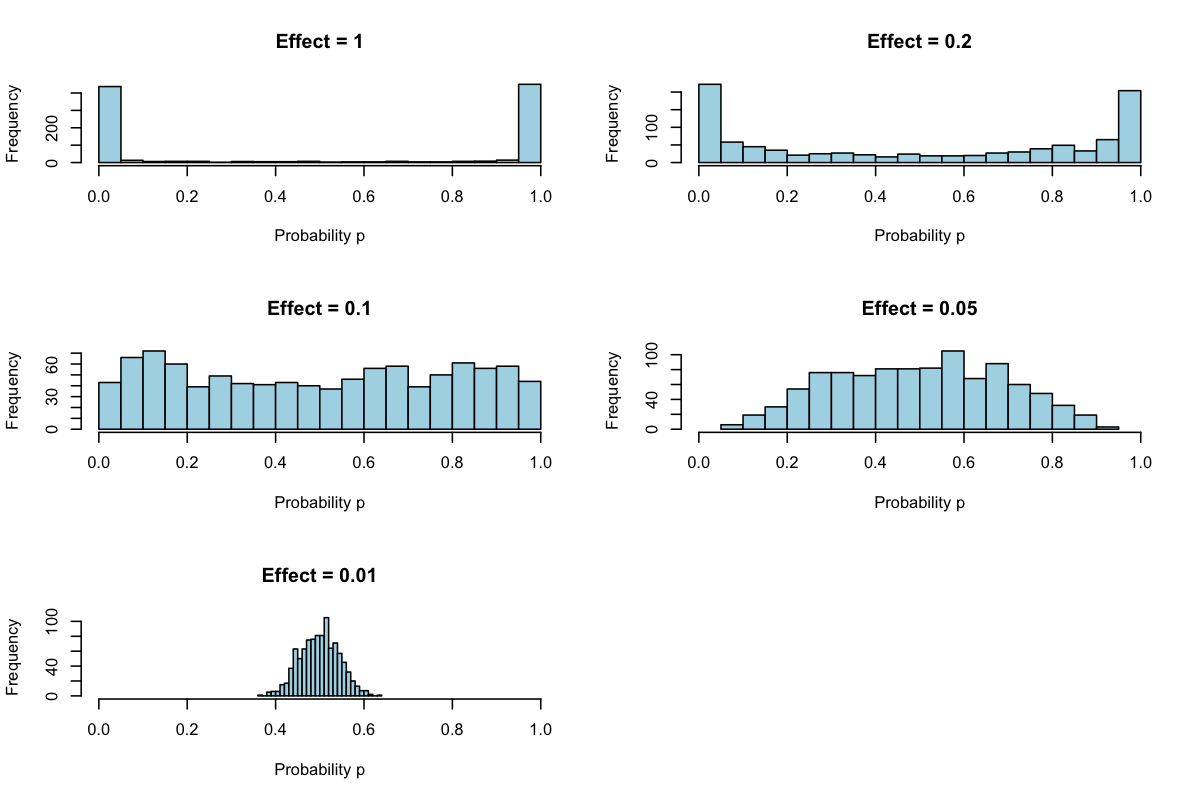
\includegraphics[width=0.8\textwidth]{sim1_p_dist.png}
  \caption{Distribution of success probability \( \mathbf{p} \) at different non-zero values in Simulation 1.}
	\label{fig:sim1_p_dist}
\end{figure}

\begin{figure}[H]
	\centering
	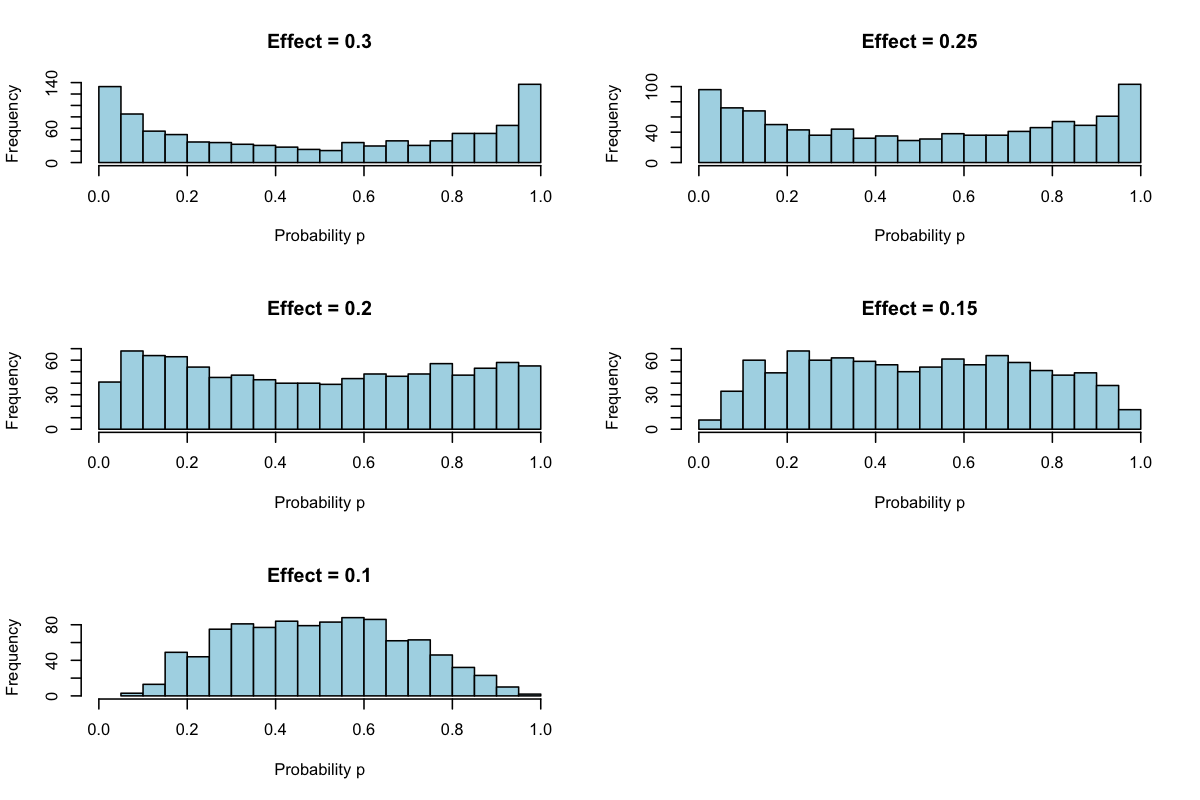
\includegraphics[width=0.8\textwidth]{sim2_p_dist.png}
  \caption{Distribution of success probability \( \mathbf{p} \) at different non-zero values in Simulation 2.}
	\label{fig:sim2_p_dist}
\end{figure}

\FloatBarrier

\subsection*{Group Mean Difference}

In this subsection, we examine the group mean differences in covariate values between instances where \( y = 1 \) and \( y = 0 \) for both Simulation 1 and Simulation 2.

Figure \ref{fig:group_diff1} presents the group mean differences for Simulation 1, with the heatmap on the left showing that regions corresponding to non-zero coefficients in \( \beta \) exhibit larger mean differences between \( y = 1 \) and \( y = 0 \), as larger covariate values in these locations have higher probabilities of being assigned to \( y = 1 \). The scatterplot on the right displays the group mean differences in the frequency domain, where each point represents a frequency component; frequencies associated with larger eigenvalues tend to have larger mean differences. Figure \ref{fig:coefs_sim1} shows the actual coefficients used in Simulation 1, where non-zero coefficients in \( \beta \) are localized to specific pixels, corresponding to the areas with larger mean differences in the group comparison.

\begin{figure}[H]
	\centering
  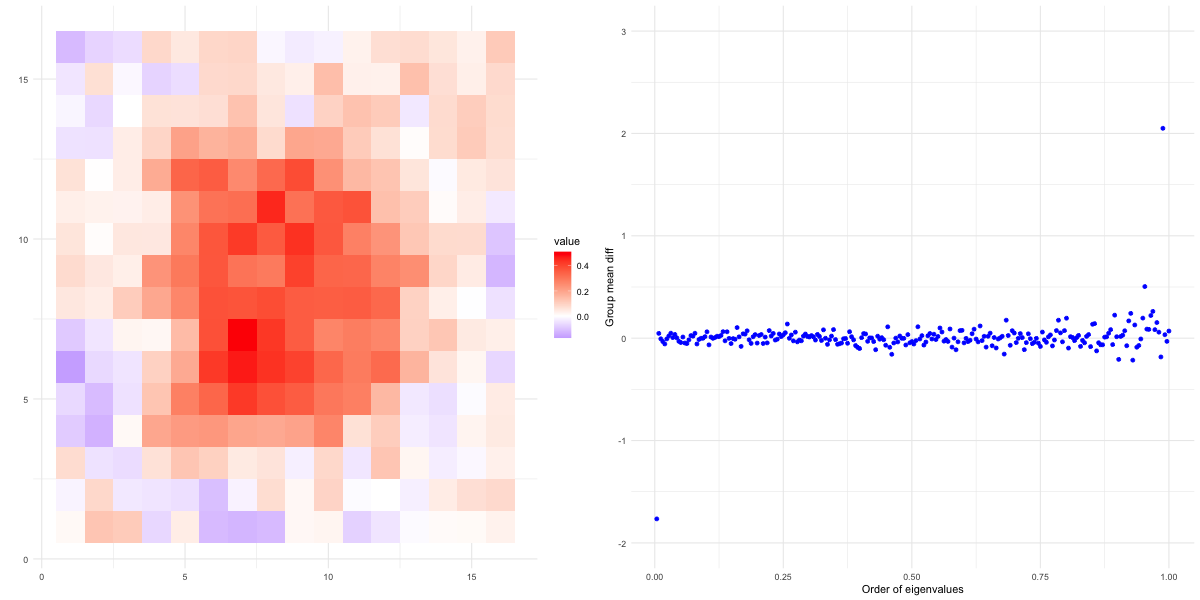
\includegraphics[width=0.8\textwidth, height=0.35\textwidth]{group_mean_diff_sim1.png}
	\caption{Group mean difference in covariate values between instances where \( y = 1 \) and \( y = 0 \) in Simulation
		1, shown for both the pixel space (left) and frequency space (right).}
	\label{fig:group_diff1}
\end{figure}

\begin{figure}[H]
	\centering
	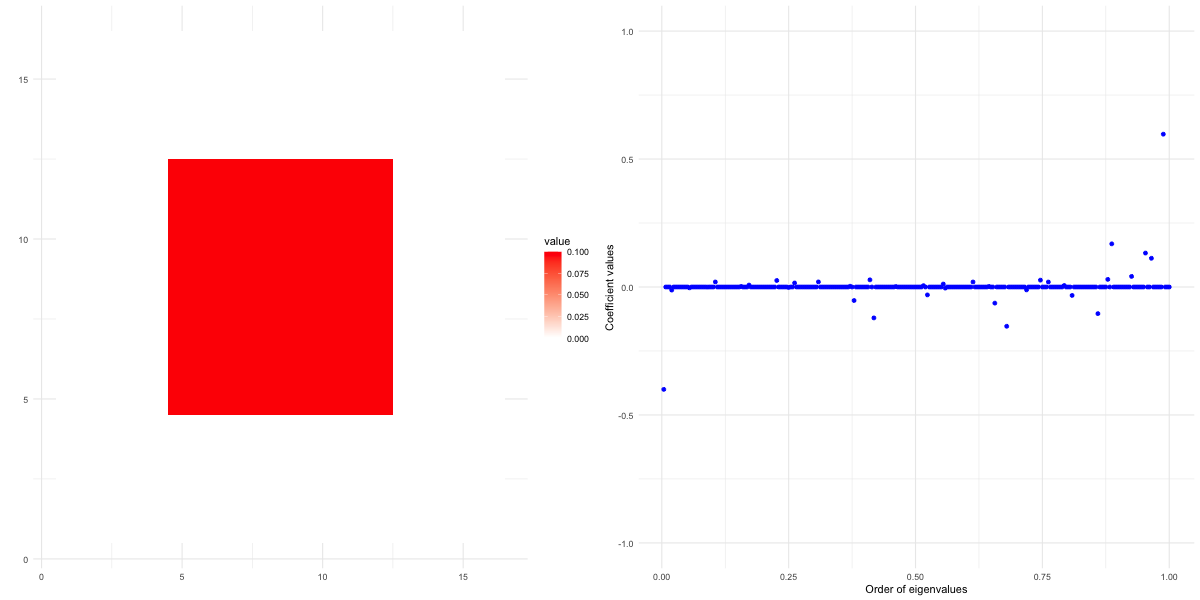
\includegraphics[width=0.8\textwidth, height=0.35\textwidth]{actual_coefs_sim1.png}
	\caption{Actual coefficients in Simulation 1 for the pixel space (left) and frequency space (right).}
	\label{fig:coefs_sim1}
\end{figure}

Figure \ref{fig:group_diff2} shows the group mean differences for Simulation 2, while Figure \ref{fig:coefs_sim2} displays the actual coefficients. The non-zero coefficients in \( \mathbf{b} \) are uniformly set to 0.2. However, the scatterplot in the frequency space does not clearly highlight the non-zero components, with increasing variance observed for larger eigenvalues. This variance pattern is consistent with the diagonal covariance matrix used in the simulation. The difficulty in identifying the non-zero components suggests that the effect size may be too small relative to the variance, making detection challenging. [Further adjustments to either the effect size or the covariance matrix could improve the detectability of these non-zero coefficients in future analyses.]

\begin{figure}[H]
	\centering
	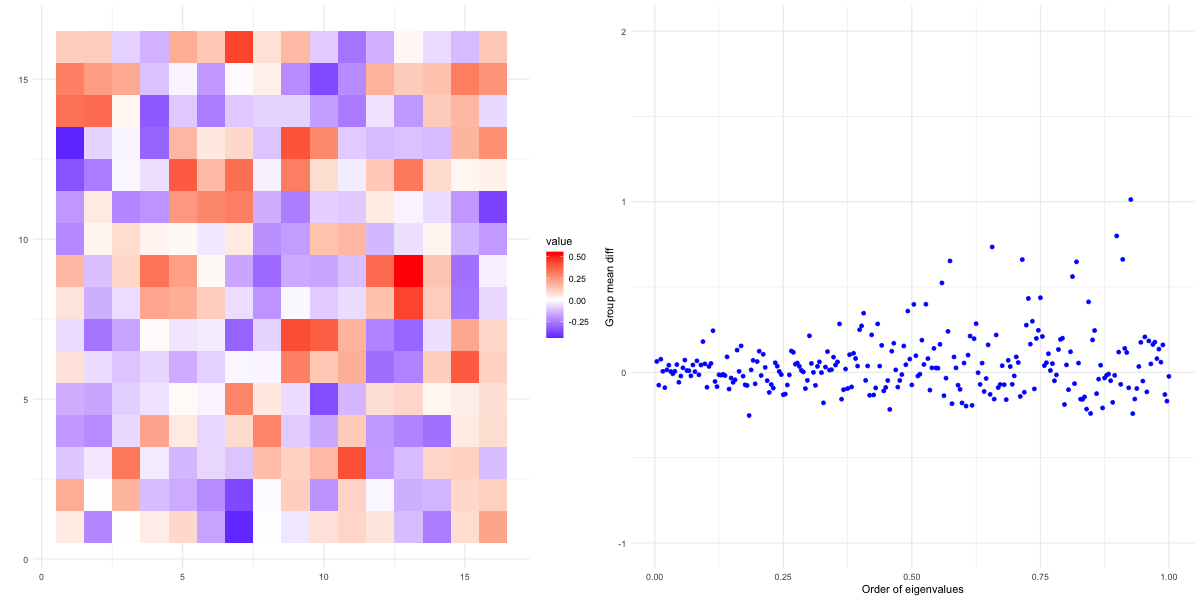
\includegraphics[width=0.8\textwidth, height=0.35\textwidth]{group_mean_diff_sim2.png}
	\caption{Group mean difference in covariate values between instances where \( y = 1 \) and \( y = 0 \) in Simulation 2.}
	\label{fig:group_diff2}
\end{figure}

\begin{figure}[H]
	\centering
	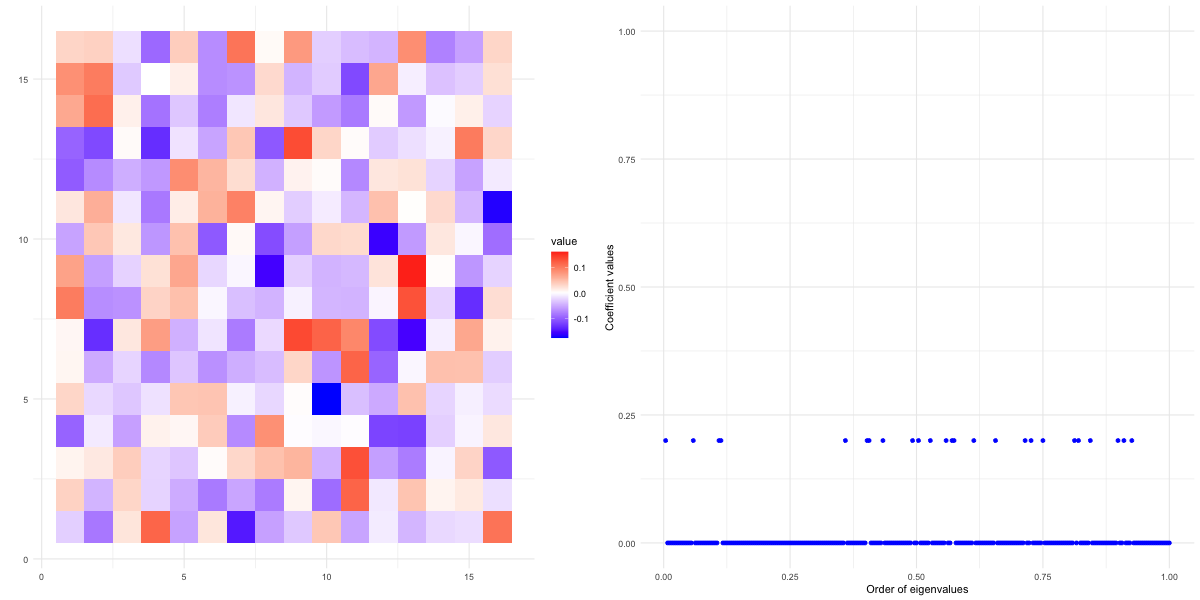
\includegraphics[width=0.8\textwidth, height=0.35\textwidth]{actual_coefs_sim2.png}
	\caption{Actual coefficients in Simulation 2 for the pixel space (left) and frequency space (right).}
	\label{fig:coefs_sim2}
\end{figure}

\FloatBarrier

\subsection*{AUC and Accuracy}

Table~\ref*{tab:auc_acc_table} summarizes the average AUCs and accuracies over 500 iterations. In both Simulation 1 (pixel space sparsity) and Simulation 2 (frequency space sparsity), models fitted in the frequency space consistently outperformed those fitted in the pixel space. For example, in Simulation 1, using \texttt{lambda.min} as the regularization parameter, models trained with pixel space covariates achieved an AUC of 0.803 (SE = 0.031) and an accuracy of 72.6\% (SE = 0.032). In contrast, models trained with frequency space covariates produced a slightly higher AUC of 0.826 (SE = 0.028) and a higher accuracy of 74.5\% (SE = 0.030). A similar trend was observed in Simulation 2, with frequency space models showing superior performance regardless of the regularization parameter used.

\begin{table}[H]
	\centering
	\caption{Comparison of AUC and accuracy between models fitted in the pixel space and frequency space across 500 iterations for Simulation 1 and Simulation 2.}
	\label{tab:auc_acc_table}
	\begin{tabular}{l|cc|cc}
		\toprule
		\textbf{Simulation}   & \multicolumn{2}{c}{\textbf{Model in Pixel Space}} & \multicolumn{2}{c}{\textbf{Model in Frequency Space}}                                              \\
		\midrule
		                      & \textbf{AUC (SE)}                                 & \textbf{Accuracy (SE)}                                & \textbf{AUC (SE)} & \textbf{Accuracy (SE)} \\
		\midrule
		\textbf{Simulation 1} &                                                   &                                                       &                   &                        \\
    \texttt{lambda.min}            & 0.803 (0.031)                                     & 0.726 (0.032)                                         & 0.826 (0.028)     & 0.745 (0.030)          \\
      \texttt{lambda.1se}            & 0.800 (0.032)                                     & 0.722 (0.032)                                         & 0.826 (0.029)     & 0.745 (0.031)          \\
		\midrule
		\textbf{Simulation 2} &                                                   &                                                       &                   &                        \\
    \texttt{lambda.min}            & 0.755 (0.036)                                     & 0.684 (0.034)                                         & 0.812 (0.030)     & 0.732 (0.032)          \\
      \texttt{lambda.1se}            & 0.735 (0.039)                                     & 0.669 (0.038)                                         & 0.812 (0.031)     & 0.732 (0.032)          \\
		\bottomrule
	\end{tabular}
\end{table}

\subsection*{Coefficients Estimation}

Figure \ref{fig:b_estimates} presents the mean estimated \( b \) values plotted against the order of eigenvalues. The order of eigenvalues are calculated the same way as above. For Simulation 1, \texttt{lambda.1se} shrinks the estimated coefficients more than \texttt{lambda.min}, as it provides a larger panelty on it. For Simulation 2, even though it is not obvious, I feel the estimated values has an increase trend as the eigenvalues increase. [Still, I am wondering whether this is related to the covariance matrix, the decreased diagonal values, consider math proof?].

The mean estimated coefficients across iterations were calculated, and Figure \ref{fig:beta_estimates} displays the mean estimated \( \beta \) values. Two key observations can be made: (1) There is no significant difference in the estimated coefficients when using \texttt{lambda.min} versus \texttt{lambda.1se}, and (2) the estimated values align well with the actual values, indicating that the model is accurately identifying the relevant features.

Figure \ref{fig:b_estimates} shows the mean estimated \( \mathbf{b} \) values plotted against the order of eigenvalues. The eigenvalue ordering is consistent with earlier calculations. In Simulation 1, \texttt{lambda.1se} applies a stronger regularization penalty, shrinking the estimated coefficients more than \texttt{lambda.min}. For Simulation 2, although the trend is less clear, there seems to be an upward trend in the estimated values as the eigenvalues increase. This trend may be related to the structure of the covariance matrix, specifically its decreasing diagonal values [consider math proof?].

\begin{figure}[H]
	\centering
	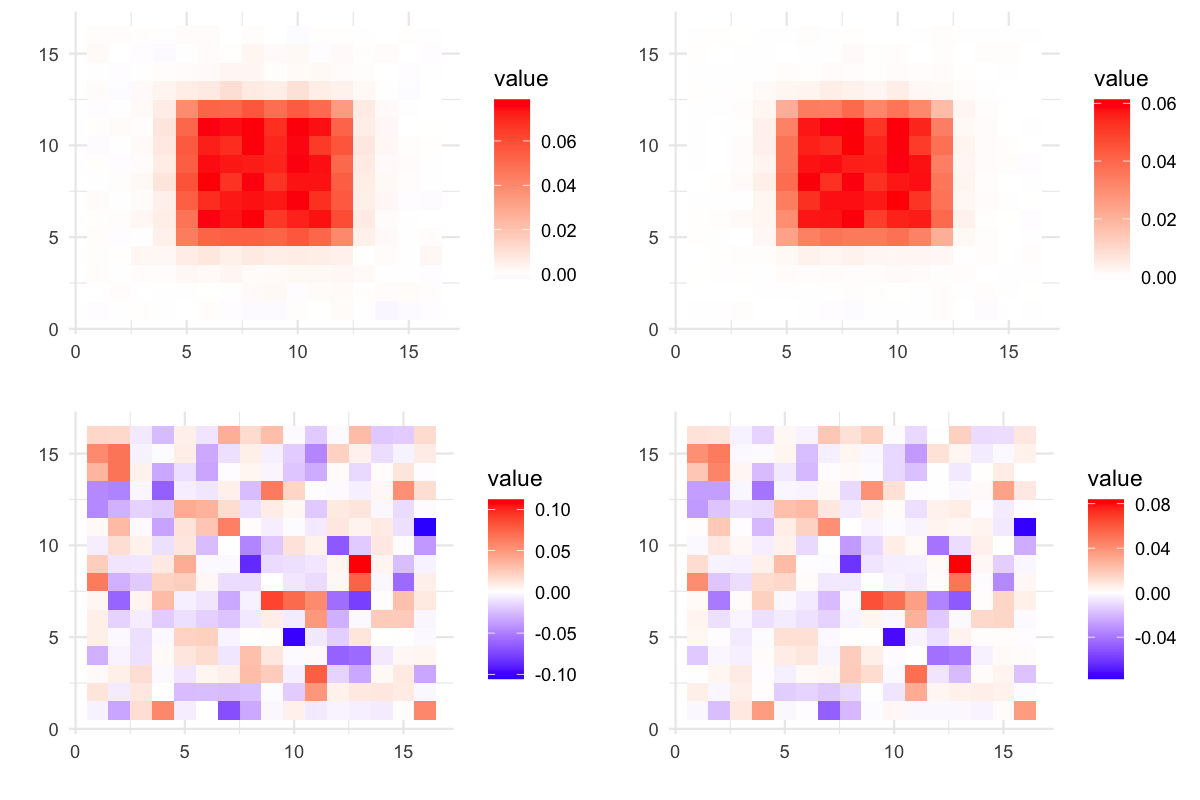
\includegraphics[width=0.8\textwidth]{beta_estimates.png}
	\caption{Mean estimated \( \beta \) values across simulations, with models fitted using \texttt{lambda.min} (left) and
		\texttt{lambda.1se} (right). The top row shows results for Simulation 1, while the bottom row shows results for Simulation 2.}
	\label{fig:beta_estimates}
\end{figure}

\begin{figure}[H]
	\centering
	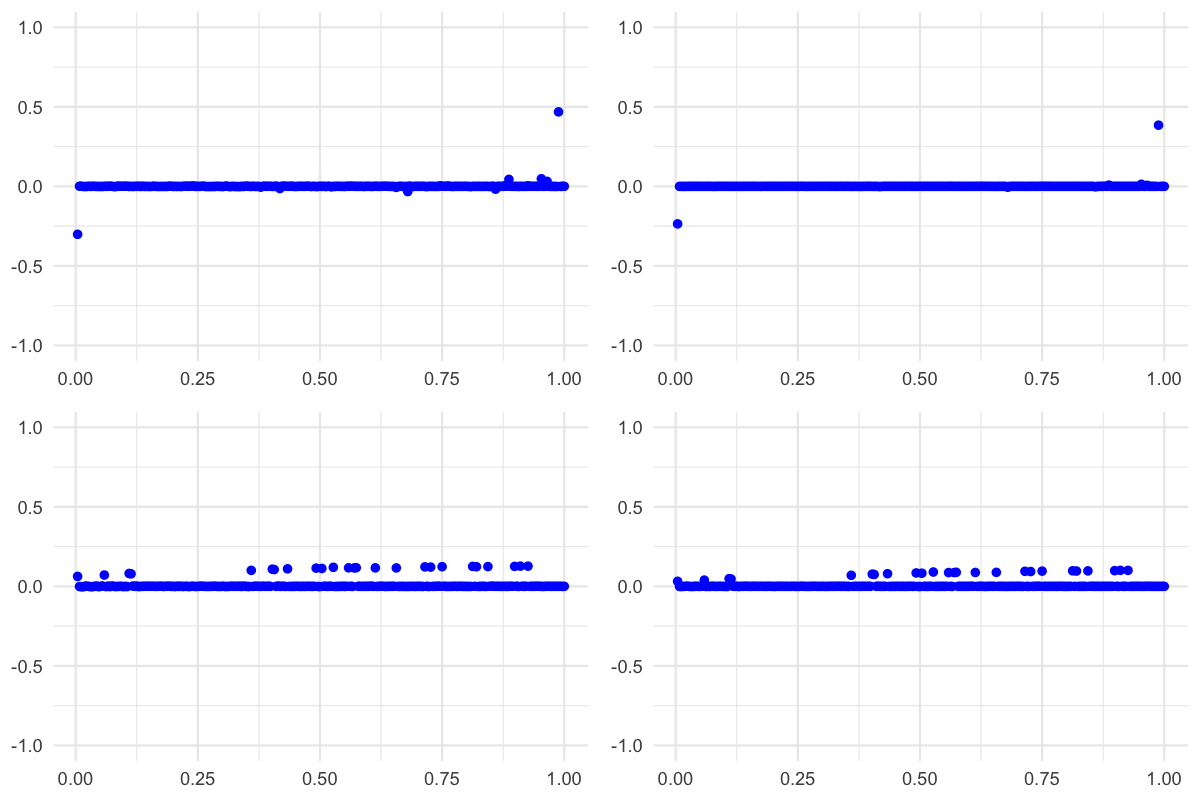
\includegraphics[width=0.8\textwidth]{b_estimates.png}
	\caption{Mean estimated \( b \) values across simulations, plotted against ordered eigenvalues. Models fitted using
		\texttt{lambda.min} are on the left and models fitted with \texttt{lambda.1se} on the right. The top row shows results for Simulation 1, while the bottom row shows results for Simulation 2.}
	\label{fig:b_estimates}
\end{figure}

\FloatBarrier

\subsection*{Significant P-values}

It is interesting to observe that, although the heatmap for significance of \( \beta \) in Simulation 1 follows the pattern of the actual non-zero values, the percentage of significance is relatively low (Figure \ref{fig:perc_sign_beta} left). In contrast, the non-zero values of \( \mathbf{b} \) (Figure \ref{fig:perc_sign_b} left) show a much higher percentage of significance, reaching as high as 100\% across iterations.

Another observation is that, although the non-zero effect size for \( \mathbf{b} \) is constant in Simulation 2, the percentage of significant p-values increases as the eigenvalues grow (Figure \ref{fig:perc_sign_b} right). [I am considering creating a plot to visualize the actual \( \beta \) values in Simulation 2 and the actual \( b \) values in Simulation 1, where the non-zero values vary, and compare them with the corresponding percentage of significant p-values. The goal is to examine whether the size of the actual non-zero values correlates with the percentage of significance. I suspect that a larger absolute effect size should result in a higher percentage of significance, but this doesn’t seem to be the case for \( b \) in Simulation 2, so I want to investigate other factors as well.]

\begin{figure}[H]
	\centering
	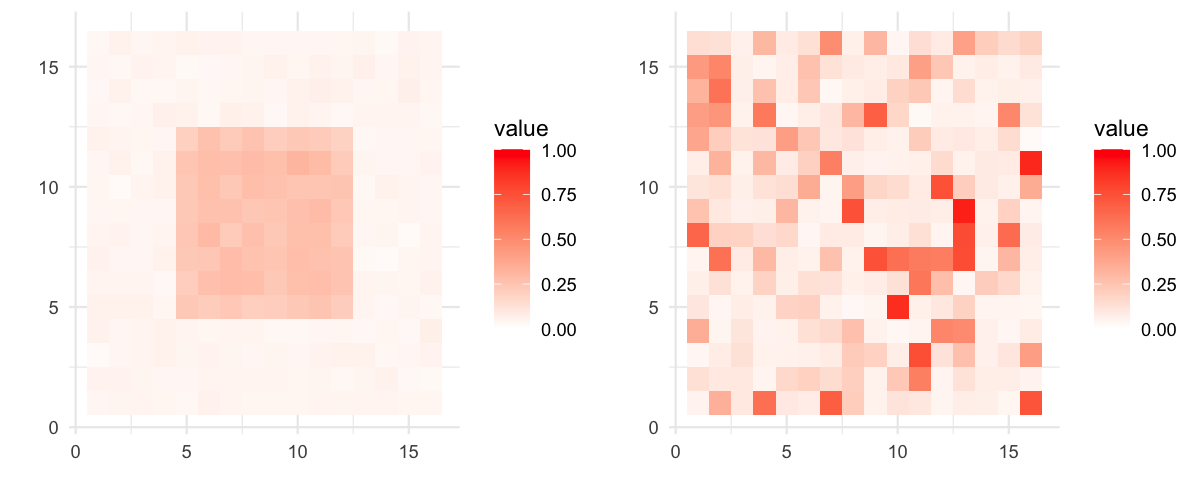
\includegraphics[width=0.9\textwidth]{perc_sign_pvals_hdi_beta.png}
	\caption{Percentage of significant p-values for elements of \( \beta \) when fitting models in the pixel space in
		Simulation 1 (left) and Simulation 2 (right).}
	\label{fig:perc_sign_beta}
\end{figure}

\begin{figure}[H]
	\centering
	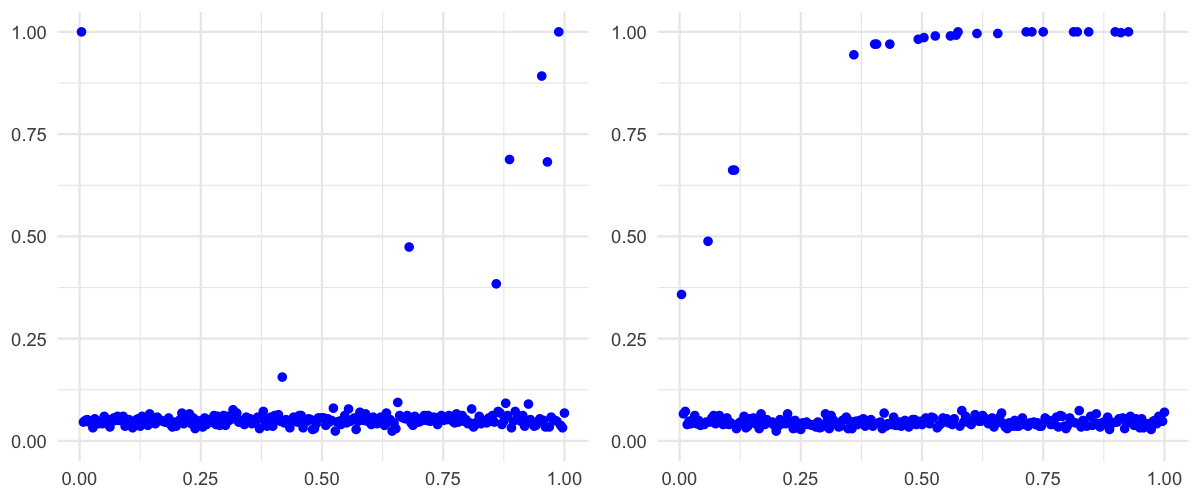
\includegraphics[width=0.9\textwidth]{perc_sign_pvals_hdi_b.png}
	\caption{Percentage of significant p-values for elements of \( b \) across ordered eigenvalues in both simulations.}
	\label{fig:perc_sign_b}
\end{figure}

\FloatBarrier


\section*{Future Work}

\begin{itemize}
  \item Adding details about how \texttt{hdi} package calculated p-values and why my permutation test didn't work.
  \item Increase \( b \) effect size (how to keep \( p \) evenly distributed in the same time?) see whether the pattern of coefficient estimates disappear or relieve.
  \item What is the next step in higher level?
\end{itemize}

\footnotesize
\bibliographystyle{abbrv}
\bibliography{references}

\end{document}


